% =============================================================
% Black-box transcripts cannot certify causal reasoning
% faithfulness in closed-API LLM agents:
% a universal observational-equivalence theorem and
% a certification-impossibility corollary.
%
% Target venue: TMLR (Transactions on Machine Learning Research)
% Source: refine-logs/FINAL_PROPOSAL.md (R5 verdict 8.42 REVISE-BUT-STOP)
%
% Uses official tmlr.sty (downloaded to tmlr-style/, version Jan 2021).
% Current shell uses article class to compile during drafting.
% =============================================================
\documentclass{article}

% TMLR style (preprint option produces a non-anonymized arXiv-ready preprint).
% Submission to OpenReview should remove the "preprint" option for double-blind.
\usepackage[preprint]{tmlr-style/tmlr}
\usepackage{amsmath,amssymb,amsfonts,amsthm,mathtools}
\usepackage{booktabs,multirow}
\usepackage{xcolor}
\usepackage{graphicx}
\usepackage{tikz}
\usetikzlibrary{arrows.meta,positioning,fit,backgrounds,calc,shapes.geometric}
\usepackage{hyperref}
\hypersetup{colorlinks=true,linkcolor=blue,citecolor=blue,urlcolor=blue}
\usepackage{microtype}
\usepackage{cleveref}

\theoremstyle{plain}
\newtheorem{theorem}{Theorem}
\newtheorem{lemma}[theorem]{Lemma}
\newtheorem{proposition}[theorem]{Proposition}
\newtheorem{corollary}[theorem]{Corollary}

\theoremstyle{definition}
\newtheorem{definition}[theorem]{Definition}
\newtheorem{assumption}[theorem]{Assumption}

\theoremstyle{remark}
\newtheorem{remark}[theorem]{Remark}

\newcommand{\TV}{\mathrm{TV}}
\newcommand{\KL}{\mathrm{KL}}
\newcommand{\NDE}{\mathrm{NDE}}
\newcommand{\dtv}{d_{\TV}}
\newcommand{\dkl}{D_{\KL}}
\newcommand{\C}{\mathcal{C}}
\newcommand{\Y}{\mathcal{Y}}
\newcommand{\YR}{\mathcal{Y}_R}
\newcommand{\YA}{\mathcal{Y}_A}
\newcommand{\Hist}{\mathcal{H}}
\newcommand{\PpiA}[1]{P_A^{\pi_{#1}}}

\title{Black-Box Transcripts Cannot Certify Causal Reasoning Faithfulness in Closed-API LLM Agents:\\
A Universal Observational-Equivalence Theorem and a Certification-Impossibility Corollary}

\author{%
  Dongcheng Zhang\thanks{Correspondence: \texttt{zdclink@gmail.com}.} \\
  BlueFocus Communication Group \\
  Beijing, China \\
  \texttt{zdclink@gmail.com}
  \AND
  Yiqing Jiang \\
  Tongji University \\
  Shanghai, China \\
  \texttt{jyq.russel@gmail.com}
}

\date{Draft \today}

\begin{document}
\maketitle

\begin{abstract}
We study external auditors that attempt to certify, from black-box transcripts
alone and \emph{over the unrestricted structural causal model class}, whether
a closed-API LLM agent's chain of reasoning is causally faithful --- in the
sense that a structural intervention on the latent reasoning state induces
a non-trivial change in the action distribution (a controlled direct effect). We formalize the audit setting as an interactive
transcript distribution under an adaptive auditor and a closed-API access
model $\mathcal{A}_0$. Our main result (Theorem~\ref{thm:transcript-indist})
is a universal observational-equivalence proposition: for every closed-API
agent $\pi_G$ with positive faithfulness, disintegration plus structural
realization exhibits a strongly compatible agent $\pi_D$ whose transcript
distribution under any adaptive auditor and any finite budget $Q$ coincides
with that of $\pi_G$, yet whose latent reasoning is causally disconnected
from the action ($L(M_D) = 0$). Theorem~\ref{thm:approx} extends this to
per-query $\varepsilon$-approximation under hybrid-occupancy reachability.
Corollary~\ref{cor:cert-imp} draws the consequence as a sharp impossibility
statement on \emph{transcript-law-only positive certificates}: over the
unrestricted SCM class no nontrivial sound such certificate exists; every
sound certificate must output zero on every realizable transcript law.
Proposition~\ref{prop:finite-alphabet} shows the decorative construction is
realizable in finite alphabets via joint-kernel distillation with explicit
sample complexity. We do not claim proof-technique novelty: the proof is
standard hybrid + DPI + Le Cam machinery applied to the LLM-agent setting.
We claim the formalization of the access-model boundary, the universal
construction, the certification-impossibility framing, and a source-checked
positioning of seven recent agent-auditing methods against the boundary. We
discuss what the theorem does \emph{not} rule out (output reliability,
action safety, retrieval grounding, white-box interpretability) and recast
three prior failed audit attempts as motivating examples rather than as
theorem validation.
\end{abstract}

% =============================================================
\section{Introduction}\label{sec:intro}

\subsection{A motivating audit scenario}

A clinical decision-support LLM agent is deployed via a closed API in a triage
pipeline. For each patient context $c$, the agent emits a pair $(Y_R, Y_A)$:
$Y_R$ is a stated chain of reasoning (``the patient's pulse and labs suggest
sepsis; therefore initiate broad-spectrum antibiotics''), and $Y_A$ is the
action (``order vancomycin + piperacillin-tazobactam''). An external auditor
--- a hospital safety committee, a regulator, a third-party assurance vendor
--- can issue any contexts $c$ it wishes and observe many $(Y_R, Y_A)$ pairs,
even adaptively (i.e., choosing the next $c$ as a function of the history). It
cannot inspect model weights, internal activations, or any latent state.
Across many such pairs the auditor wants to draw a specific conclusion: that
the stated reasoning $Y_R$ is a \emph{causally faithful} report of the
internal computation that produced $Y_A$, in the sense that the latent
reasoning state $R$ that the model used has a non-zero direct effect on
$Y_A$ in the model's underlying structural causal mechanism. If $Y_R$ were
generated by a process structurally disconnected from the mechanism that
produced $Y_A$ --- e.g., a post-hoc explanation generator that conditions on
$Y_A$ rather than producing it --- the agent would be \emph{decorative} in
the technical sense we adopt: its reasoning narration is correlated with its
actions but does not causally drive them. The auditor would like a
\emph{certificate} that distinguishes the two cases. This paper proves that,
under the closed-API access model, no such certificate exists at the level of
generality usually asked for.

\subsection{What we prove}

We formalize the audit setting as an interactive transcript distribution
$P_A^\pi(T_Q)$ generated by an adaptive auditor $A$ and a closed-API agent
$\pi$ over $Q$ rounds (\Cref{def:agent,def:auditor,def:A0}, depicted in
\Cref{fig:auditor-loop}). We then prove three connected results.

\begin{enumerate}
  \item \textbf{Universal observational-equivalence}
    (Theorem~\ref{thm:transcript-indist}). For every faithful agent $\pi_G$
    with $L(M_G) > 0$, the disintegration of its observable channel
    (Lemma~\ref{lem:A}) plus structural noise-outsourcing
    (Lemma~\ref{lem:B}) yields a strongly compatible decorative agent
    $\pi_D$ whose per-history kernel coincides with $\pi_G$'s while its
    latent reasoning state has no structural arrow into the action. This
    is a \emph{representation theorem}: the decorative twin is constructed,
    not merely asserted to exist (\Cref{fig:counterexample}).
  \item \textbf{Approximate version} (Theorem~\ref{thm:approx}). When $\pi_D$
    is replaced by a $\varepsilon$-TV-close approximation $\pi_D^\varepsilon$
    on the auditor's hybrid-occupancy support, the transcript-law gap is at
    most $\min(1, Q\varepsilon)$ for every adaptive auditor and budget $Q$.
  \item \textbf{Certification impossibility}
    (Corollary~\ref{cor:cert-imp}). Over the unrestricted SCM class, no
    nontrivial sound transcript-law-only positive certificate for the
    faithfulness property exists; every sound certificate must output
    zero on every realizable transcript law.
\end{enumerate}

A finite-alphabet realizability proposition
(Proposition~\ref{prop:finite-alphabet}) shows that $\pi_D^\varepsilon$ can
be obtained by joint-kernel distillation from samples of $\pi_G$, with
explicit sample complexity, defusing the natural ``oracle-flavored
construction'' objection. A small synthetic experiment
(\Cref{app:validation}, \Cref{fig:auc-curve}) illustrates that the
$Q\varepsilon$ degradation shape is empirically observable in a controlled
finite setting.

\subsection{What we do \emph{not} prove}

The theorem rules out a specific class of certificates --- those that depend
only on the transcript law and must be sound over the unrestricted SCM class.
It does not say that black-box auditing is invalid in general. Output
reliability on verifiable subtasks, action-safety properties, retrieval
grounding, robustness to prompt injection, and benchmark accuracy are all
auditable from black-box transcripts; their identification targets simply
differ from latent causal reasoning faithfulness. White-box interpretability
methods that intervene on internal activations \citep{geiger2022inducing,
geiger2023causal} use a strictly stronger access model ($\mathcal{A}_W$) and
are outside our boundary. \Cref{sec:not-said} catalogs these distinctions
prominently to forestall the common overread that the result proves
something stronger than it does. Several recent agent-auditing methods are
\emph{often interpreted} as evidence about reasoning faithfulness even though
their original papers frame the claim more modestly; \Cref{tab:access-table}
positions seven such methods against our boundary based on a direct
source-check, with one PARTIAL and six NO labels and no YES.

\subsection{Why this is a contribution despite using standard machinery}

The proof is standard: disintegration on Polish spaces
\citep{kallenberg2021}, noise outsourcing as Borel iso plus quantile
\citep{kallenberg2021}, adaptive hybrid arguments, data-processing inequality,
Le Cam's two-point method \citep{lecam1986,tsybakov2009}. We do not claim
proof-technique novelty. The contribution is fourfold: \emph{(i)} formalizing
\emph{causal reasoning faithfulness} as a latent SCM property
(Definition~\ref{def:L}) in the LLM-agent setting; \emph{(ii)} naming the
closed-API access model $\mathcal{A}_0$ and locating the boundary it draws;
\emph{(iii)} exhibiting a universal disintegration-based decorative twin
construction $\pi_G \mapsto \pi_D$ that converts the existential
non-identifiability statement into a representation theorem; and \emph{(iv)}
deriving Corollary~\ref{cor:cert-imp} as a sharp impossibility statement on
\emph{all} transcript-law-only certificates rather than on a single
distinguishing test, including a precise definition of certificate semantics
that addresses the philosophical objection that a Bayesian or assumption-
restricted auditor might recover identifiability by other means.

\subsection{Roadmap}

\Cref{sec:notss} fixes notation and the agent/auditor/access-model setup.
\Cref{sec:not-said} catalogs what the theorem does \emph{not} say.
\Cref{sec:lem-A,sec:lem-B} develop the kernel-realization toolkit.
\Cref{sec:thm-1} states and proves the universal observational-equivalence
theorem and its definitional caveat. \Cref{sec:approx} gives the
approximate version. \Cref{sec:cor-1} states the certification-impossibility
corollary preceded by a Certificate Semantics paragraph.
\Cref{sec:prop-1} gives the finite-alphabet realizability proposition.
\Cref{sec:empirical} recasts three prior audit attempts as motivating
examples and includes one new closed-API LLM snapshot.
\Cref{sec:access-table} contains the source-checked positioning of recent
agent-auditing work. \Cref{sec:relwork} discusses related work in three
adjacent threads. \Cref{sec:discussion} addresses scope, escape hatches,
limitations. \Cref{sec:conclusion} concludes. Appendices contain proofs of
\Cref{lem:A,lem:B}, the uniform variant of Theorem~\ref{thm:approx},
the KL-refinement lemma, and the validation experiment.

% =============================================================
\section{What Theorem~\ref{thm:transcript-indist} does not say}\label{sec:not-said}

% R5 reviewer: "the 'What Theorem 1 Does Not Say' box is important and should remain."
We list, prominently and early, what the impossibility result does \emph{not} prove,
to forestall the common overread that the paper rules out all auditing.

\begin{itemize}
  \item Output reliability is unauditable. (Action correctness on verifiable subtasks IS auditable.)
  \item Reasoning text is meaningless. (Plausibility under task-relevance metrics IS measurable.)
  \item Action safety is unauditable. (Action-policy properties testable from samples ARE auditable.)
  \item Benchmark accuracy is unauditable. (Standard ML eval is fine.)
  \item Post-hoc explanation quality is meaningless. (It is a different property: \emph{plausibility} of $Y_R$, not \emph{causal faithfulness} of $R$.)
  \item Internal-state interpretability is impossible. (White-box access $\mathcal{A}_W$ admits identification.)
  \item Trustworthy reasoning is hopeless. (It requires stronger access, instrumented architectures, or task-verifiable reasoning.)
  \item The cited prior work claims to certify faithfulness. (We say: those methods \emph{are often interpreted} as evidence about faithfulness; our result formalizes a boundary on what such evidence can certify.)
\end{itemize}

The theorem proves a \emph{specific} boundary: the latent causal-faithfulness
property of $R$ on $Y_A$ cannot be certified from the full adaptive transcript
law generated by the black-box channel, over the \emph{unrestricted} SCM class.

% =============================================================
\section{Notation and Setting}\label{sec:notss}

We work on standard Borel measurable spaces $(\C, \mathcal{F}_C)$,
$(\YR, \mathcal{F}_R)$, $(\YA, \mathcal{F}_A)$. Joint output $\Y = \YR \times \YA$.
Finite horizon $Q < \infty$. The history space
$\Hist_{\le t-1} := (\C \times \Y)^{t-1}$ is standard Borel by finite product
closure; we write $\Hist_Q := (\C \times \Y)^Q$ for the full transcript
space at budget $Q$. The Borel $\sigma$-algebras are denoted $\mathcal F_C$,
$\mathcal F_R$, $\mathcal F_A$ for $\C, \YR, \YA$ respectively, with
$\mathcal F_Y := \mathcal F_R \otimes \mathcal F_A$ on $\Y = \YR \times \YA$.

\begin{definition}[Closed-API agent]\label{def:agent}
A \emph{closed-API agent} $\pi$ is a family of measurable stochastic kernels
$\{K_{\pi, t}\}_{t \ge 1}$ where each
$K_{\pi, t} : \C \times \Hist_{\le t-1} \to \mathcal{P}(\Y)$ satisfies the
joint-measurability condition that, for every $B \in \mathcal F_Y$, the
map $(c, h) \mapsto K_{\pi, t}(B \mid c, h)$ is
$\mathcal F_C \otimes \mathcal F_{\Hist_{\le t-1}}$-measurable. The
stateless special case is $K_{\pi, t}(\cdot \mid c, h) = K_\pi(\cdot \mid c)$
independent of $t$ and $h$. We write $K_\pi$ when the $t$-index is
implicit from context. Auditing is parameterized by a budget $Q < \infty$
chosen at evaluation time; the kernel family is defined for every $t$ so
that strong-compatibility statements over $\mathcal Q$ are well-typed.
\end{definition}

\begin{definition}[Adaptive auditor]\label{def:auditor}
An \emph{adaptive auditor} is a family of measurable randomized kernels
$\{A_t\}_{t \ge 1}$ with $A_t : \Hist_{\le t-1} \to \mathcal{P}(\C)$
satisfying the analogous joint-measurability condition. We write $A$ for
the family.
\end{definition}

The \emph{transcript law} under budget $Q$ is the law of
$T_Q = ((c_1, y_1), \ldots, (c_Q, y_Q))$ on $(\C \times \Y)^Q$ obtained
by the Ionescu-Tulcea construction
\citep[Theorem~6.16]{kallenberg2021}: alternately apply $A_t$ to draw
$c_t$, then $K_{\pi, t}$ to draw $y_t = (y_{R, t}, y_{A, t})$, conditioned
on the prior history $h_{t-1}$.

\begin{definition}[Causal reasoning faithfulness]\label{def:L}
Let $M_\pi = (V, U, \mathcal{F}, P_U)$ be a latent SCM realizing $K_\pi$
through the structural representation of \Cref{lem:B}, with a designated
latent reasoning variable $R_t$ at each round $t$. For each $r \in \mathcal R_t$
(the state space of $R_t$), define the \emph{interventional structural kernel}
\[
K^{M_\pi,\, do(R_t = r)}_{A, t}(\,\cdot \mid c, h)
\;\;:\;\;
\C \times \Hist_{\le t-1} \to \mathcal P(\Y_A),
\]
obtained by replacing the $R_t$ argument in the structural equation
$Y_{A,t} = f_{A,t}(c, h, R_t, U_{A,t})$ with the constant $r$ and
marginalizing the remaining exogenous noise. The \emph{faithfulness
indicator} is then
\[
L(M_\pi) \;:=\; \sum_{t=1}^Q \mathbf{1}\!\Big[
  \exists\, r, r' \in \mathcal R_t \;:\;
  K^{M_\pi,\, do(R_t = r)}_{A, t} \;\not\equiv\;
  K^{M_\pi,\, do(R_t = r')}_{A, t}
\Big],
\]
where $\not\equiv$ means \emph{pointwise inequality of Markov kernels}:
there exist $(c, h) \in \C \times \Hist_{\le t-1}$ and $B \in \mathcal F_A$
such that
$K^{M_\pi, do(R_t = r)}_{A, t}(B \mid c, h) \neq K^{M_\pi, do(R_t = r')}_{A, t}(B \mid c, h)$.

\smallskip
$L(M_\pi) > 0$ iff at some round $t$, the structural intervention $do(R_t)$
induces a non-trivial change in the action kernel. This is a
\emph{controlled direct effect} in the structural sense: we hold the
upstream context-history fixed and intervene on $R_t$ only, with no
cross-world quantities involved. We do not claim equivalence to natural
direct effect \citep{pearl2001direct}; the structural-arrow form is what
\Cref{thm:transcript-indist}(ii) actually proves to be zero in the
decorative SCM, and this is the form we use throughout.
\end{definition}

\begin{definition}[Closed-API access model $\mathcal{A}_0$]\label{def:A0}
Auditor observes only $(Y_R, Y_A)$ samples from $K_\pi$; no internal-state
oracle, no $\mathit{do}$-interventions on latent variables.
\end{definition}

\begin{figure}[ht]
\centering
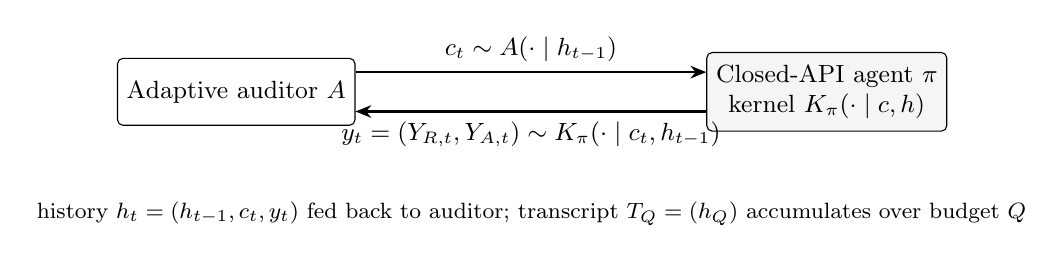
\begin{tikzpicture}[
  >={Stealth[length=2.0mm,width=1.6mm]},
  every node/.style={font=\small},
  box/.style={draw, rounded corners=2pt, minimum width=22mm, minimum height=8.5mm, align=center},
  ag/.style={draw, fill=black!4, rounded corners=2pt, minimum width=24mm, minimum height=10mm, align=center},
  arr/.style={->, thick},
]
  \node[box] (A) at (0,0) {Adaptive auditor $A$};
  \node[ag]  (P) at (7.5,0) {Closed-API agent $\pi$\\ kernel $K_\pi(\cdot \mid c, h)$};
  \draw[arr] ($(A.east) + (0,0.25)$) -- node[above]{$c_t \sim A(\cdot \mid h_{t-1})$} ($(P.west) + (0,0.25)$);
  \draw[arr] ($(P.west) + (0,-0.25)$) -- node[below]{$y_t = (Y_{R,t}, Y_{A,t}) \sim K_\pi(\cdot \mid c_t, h_{t-1})$} ($(A.east) + (0,-0.25)$);
  \node[align=center, font=\footnotesize] at (3.75,-1.55)
    {history $h_t = (h_{t-1}, c_t, y_t)$ fed back to auditor; transcript $T_Q = (h_Q)$ accumulates over budget $Q$};
\end{tikzpicture}
\caption{Adaptive auditor--agent interaction under access model $\mathcal{A}_0$
(Definitions~\ref{def:auditor}--\ref{def:A0}). The auditor's only observation is
the per-query pair $(Y_R, Y_A)$; the latent reasoning state $R$ is never
observed and never intervened on.}
\label{fig:auditor-loop}
\end{figure}

\begin{definition}[Strong compatibility]\label{def:compat}
SCMs $M, M'$ are \emph{strongly compatible} (with respect to a class
$\mathfrak{A}$ of measurable adaptive auditors and a finite-budget set
$\mathcal Q \subseteq \mathbb N$) iff for every $A \in \mathfrak{A}$ and
every $Q \in \mathcal Q$, the induced transcript laws coincide:
\[
P_A^M(T_Q) \;=\; P_A^{M'}(T_Q) \quad \text{as probability measures on } (\C \times \Y)^Q.
\]
We refer to the transcript-law definition as the \emph{primary} formulation.

\smallskip
A simple \emph{sufficient condition} for strong compatibility against the
class of all measurable adaptive auditors and every budget $Q \le Q_{\max}$
is pointwise kernel equality: there exist regular conditional versions
$K_{M,t}$ and $K_{M',t}$ such that for every
$t \in \{1, \ldots, Q_{\max}\}$ and every
$(c, h) \in \C \times \Hist_{\le t-1}$,
$K_{M,t}(\cdot \mid c, h) = K_{M',t}(\cdot \mid c, h)$. The decorative
construction of \Cref{thm:transcript-indist} delivers this stronger condition
directly, after which \Cref{thm:transcript-indist}(iv) gives transcript-law
equality by Ionescu-Tulcea induction. Strong compatibility is a strictly
weaker requirement (auditors only probe kernels on the histories they
actually reach, so kernel disagreement off the auditor-induced occupancy
support cannot be detected); we do not need the weaker form for the main
result.
\end{definition}

% =============================================================
\section{Lemma A: Kernel Factorization}\label{sec:lem-A}

\begin{lemma}[Disintegration]\label{lem:A}
For any standard Borel parameter space $X = \C \times \Hist$ and output space
$\YR \times \YA$, a Markov kernel $K_G(dy_R, dy_A \mid x)$ admits a measurable
regular conditional kernel $K_G(dy_R \mid x, y_A)$ with respect to the marginal
$K_G(dy_A \mid x)$, satisfying
\[
K_G(dy_R, dy_A \mid x) = K_G(dy_A \mid x) \cdot K_G(dy_R \mid x, y_A).
\]
The factorization is $K_G(dy_A \mid x)$-almost-everywhere unique.
\end{lemma}
\begin{proof}[Reference]
Standard application of disintegration on Polish spaces; see
\citet[Theorem~8.5]{kallenberg2021}. Full statement in
\Cref{app:lem-A-proof}.
\end{proof}

% =============================================================
\section{Lemma B: SCM Realization via Noise Outsourcing}\label{sec:lem-B}

\begin{lemma}[Measurable structural representation]\label{lem:B}
Every standard Borel stochastic kernel $K(dy \mid x)$ admits a measurable
structural representation: there exist a standard Borel exogenous noise space
$(\mathcal{U}, P_U) = ([0,1], \mathrm{Leb})$ and a measurable function
$f : X \times \mathcal{U} \to \Y$ such that $Y = f(x, U)$ with $U \sim P_U$
implies $P(Y \in B \mid X = x) = K(B \mid x)$.
\end{lemma}
\begin{proof}[Reference]
Measurable-randomization / noise-outsourcing for Markov kernels on standard
Borel spaces; see \citet[Theorem~6.10 and Lemma~4.22]{kallenberg2021} or the
self-contained Borel-isomorphism + quantile argument in \Cref{app:lem-B-proof}.
\end{proof}

% =============================================================
\section{Theorem 1: Transcript Indistinguishability}\label{sec:thm-1}

\begin{assumption}\label{ass:standard-borel}
$\C, \YR, \YA$ are standard Borel spaces and the horizon $Q$ is finite.
\end{assumption}

\begin{assumption}\label{ass:auditor}
The auditor $A$ is a measurable randomized kernel.
\end{assumption}

\begin{theorem}[Universal Observational Equivalence]\label{thm:transcript-indist}
Fix any closed-API agent $\pi_G$ with kernel $K_G$ and latent SCM $M_G$ such
that $L(M_G) > 0$. Under \Cref{ass:standard-borel,ass:auditor}, there exists
a closed-API agent $\pi_D$ with kernel $K_D$ and latent SCM $M_D$ such that:
\begin{enumerate}
  \item[(i)] \emph{Per-round conditional independence:}
    $R_t^D \perp Y_{A,t} \mid C_t, H_{t-1}$ for all $t$.
  \item[(ii)] \emph{Faithfulness gap:} $L(M_D) = 0$.
  \item[(iii)] \emph{Strong compatibility:}
    $K_D(\cdot \mid c, h) = K_G(\cdot \mid c, h)$ for all reachable $(c, h)$.
  \item[(iv)] \emph{Universal transcript equality:} for any adaptive auditor
    $A$ and any budget $Q$,
    \[
    \PpiA{G}(T_Q) = \PpiA{D}(T_Q).
    \]
  \item[(v)] \emph{Le Cam consequence:} any test
    $\psi : \Hist_Q \to \{G, D\}$ has total error
    \[
    \inf_\psi \big( \Pr_{\pi_G}[\psi = D] + \Pr_{\pi_D}[\psi = G] \big)
    = 1 - \dtv\big(\PpiA{G}(T_Q), \PpiA{D}(T_Q)\big) = 1.
    \]
\end{enumerate}
\end{theorem}

\begin{figure}[ht]
\centering
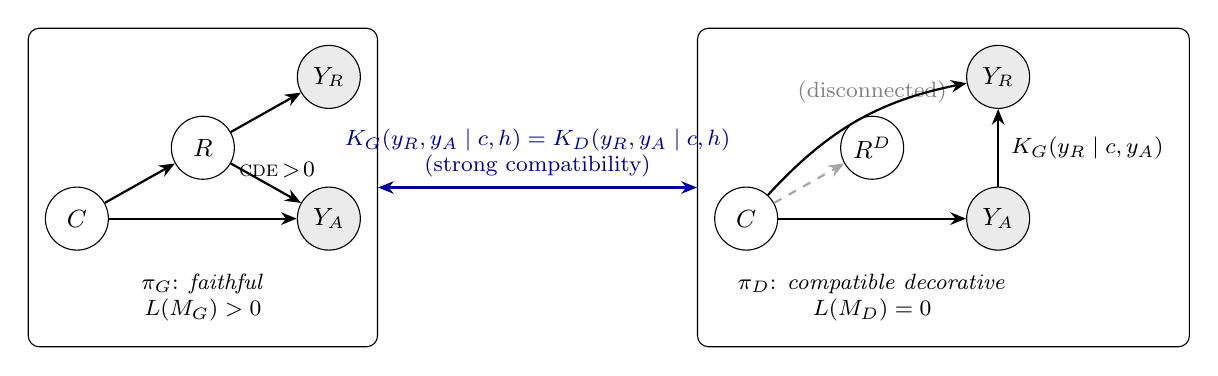
\begin{tikzpicture}[
  >={Stealth[length=2.0mm,width=1.6mm]},
  every node/.style={font=\small},
  var/.style={draw, circle, minimum size=8mm, inner sep=0pt},
  exo/.style={draw, dashed, circle, minimum size=7mm, inner sep=0pt, font=\footnotesize},
  arr/.style={->, thick},
  faded/.style={->, thick, dashed, gray!70},
  panel/.style={draw, rounded corners=4pt, inner sep=6pt},
  obs/.style={fill=black!8},
]
  % ---------- Left panel: pi_G (faithful) ----------
  \begin{scope}[local bounding box=Gpanel]
    \node[var]               (cG) at (0, 0)     {$C$};
    \node[var]               (rG) at (1.6, 0.9) {$R$};
    \node[var, obs]          (yaG) at (3.2, 0)  {$Y_A$};
    \node[var, obs]          (yrG) at (3.2, 1.8){$Y_R$};
    \draw[arr] (cG) -- (rG);
    \draw[arr] (cG) -- (yaG);
    \draw[arr] (rG) -- (yaG)
      node[midway, above, sloped=false, xshift=4pt, yshift=-2pt, font=\footnotesize]{\textsc{cde}\,$>\!0$};
    \draw[arr] (rG) -- (yrG);
    \node[font=\footnotesize, align=center] at (1.6, -1.0)
      {$\pi_G$: \emph{faithful}\\ $L(M_G) > 0$};
  \end{scope}
  \node[panel, fit=(Gpanel) (cG) (rG) (yrG)] (Gbox) {};

  % ---------- Right panel: pi_D (decorative) ----------
  \begin{scope}[xshift=8.5cm, local bounding box=Dpanel]
    \node[var]               (cD)  at (0, 0)     {$C$};
    \node[var]               (rD)  at (1.6, 0.9) {$R^D$};
    \node[var, obs]          (yaD) at (3.2, 0)   {$Y_A$};
    \node[var, obs]          (yrD) at (3.2, 1.8) {$Y_R$};
    \draw[arr] (cD) -- (yaD);
    \draw[faded] (cD) -- (rD);
    \node[font=\footnotesize, gray, above=1pt of rD]{(disconnected)};
    \draw[arr] (yaD) -- (yrD)
      node[midway, right=1pt, font=\footnotesize]
        {$K_G(y_R \mid c, y_A)$};
    \draw[arr] (cD) to[bend left=18] (yrD);
    \node[font=\footnotesize, align=center] at (1.6, -1.0)
      {$\pi_D$: \emph{compatible decorative}\\ $L(M_D) = 0$};
  \end{scope}
  \node[panel, fit=(Dpanel) (cD) (rD) (yrD)] (Dbox) {};

  % equality between observable channels
  \draw[<->, thick, blue!60!black]
    (Gbox.east) -- (Dbox.west)
    node[midway, above, font=\footnotesize, align=center, blue!60!black]
      {$K_G(y_R, y_A \mid c, h) = K_D(y_R, y_A \mid c, h)$\\(strong compatibility)};
\end{tikzpicture}
\caption{Counterexample construction (Theorem~\ref{thm:transcript-indist}).
\textbf{Left}: faithful agent $\pi_G$ with latent reasoning state $R$ that
causally drives $Y_A$ (controlled direct effect $> 0$, equivalently $L(M_G) > 0$) and is reported via $Y_R$.
\textbf{Right}: compatible decorative agent $\pi_D$ obtained by disintegration
plus structural realization (Lemmas~\ref{lem:A}--\ref{lem:B}). $Y_A$ is
generated directly from $C$ with no $R^D$ argument, so $L(M_D) = 0$;
$Y_R$ is then sampled from the regular conditional $K_G(y_R \mid c, y_A)$
\emph{after} $Y_A$ is fixed. Observed nodes are shaded; the latent $R^D$ in
$\pi_D$ is causally disconnected from $Y_A$ (dashed edge omitted from any
parent of $Y_A$). Both panels induce the \emph{same} observable channel.}
\label{fig:counterexample}
\end{figure}

\paragraph{Construction of $\pi_D$.}
For every $t \ge 1$ (so that the construction works at every finite budget):
\begin{enumerate}
\item By \Cref{lem:A}, factor
$K_G(dy_R, dy_A \mid c_t, h_{t-1}) = K_G(dy_A \mid c_t, h_{t-1}) \cdot K_G(dy_R \mid c_t, y_A, h_{t-1})$.
\item By \Cref{lem:B}, realize each factor as a measurable structural equation:
\begin{align*}
Y_{A,t} &= f_{A,t}^D(c_t, h_{t-1}, U_{A,t}'),\\
R_t^D &= f_{R,t}^D(c_t, h_{t-1}, U_{R,t}'),\\
Y_{R,t} &= f_{Y_R,t}^D(c_t, h_{t-1}, Y_{A,t}, U_{E,t}'),
\end{align*}
where $f_{A,t}^D$ realizes $K_G(dy_A \mid c_t, h_{t-1})$, $f_{R,t}^D$ realizes
any chosen distribution for the latent reasoning variable, and $f_{Y_R,t}^D$
realizes $K_G(dy_R \mid c_t, y_A, h_{t-1})$.
\end{enumerate}
The exogenous noise families $\{U_{A,t}', U_{R,t}', U_{E,t}'\}_{t \ge 1}$ are
mutually independent across all $t$ and all three families. \emph{Critical:}
$f_{A,t}^D$ does not take $R_t^D$ (or $U_{R,t}'$) as argument.

\paragraph{Sketch of proofs (full proofs immediately below in \Cref{sec:thm-1-proofs}).}
(i) follows from independence of the exogenous noise $U_{A,t}'$ and $U_{R,t}'$.
(ii) follows from the structural intervention argument:
$f_{A,t}^D$ has no $R_t^D$ argument, so $\mathit{do}(R_t^D = r)$ leaves $Y_{A,t}$
unchanged for every $r$, hence the structural-arrow indicator at round $t$ is zero, and $L(M_D) = \sum_t 0 = 0$.
(iii) follows from \Cref{lem:A} applied to both $K_G$ and $K_D$.
(iv) follows from (iii) by induction on $t$.
(v) is Le Cam's two-point method with $\dtv = 0$.

\subsection{Proofs of Theorem~\ref{thm:transcript-indist}}\label{sec:thm-1-proofs}

\begin{proof}[Proof of (i)]
By construction $f_{A,t}^D$ does not take $U_{R,t}'$ as input, so $Y_{A,t}$ is
a measurable function of $(c_t, h_{t-1}, U_{A,t}')$. Similarly $R_t^D$
depends only on $(c_t, h_{t-1}, U_{R,t}')$. By independence of $U_{A,t}'$ and
$U_{R,t}'$, conditioning on $(C_t, H_{t-1})$ leaves $R_t^D \perp Y_{A,t}$.
\end{proof}

\begin{proof}[Proof of (ii)]
By construction the structural equation $Y_{A,t} = f_{A,t}^D(c_t, h_{t-1}, U_{A,t}')$
does not take $R_t^D$ as an argument. Hence the interventional structural
kernel $K^{M_D, do(R_t^D = r)}_{A, t}(\cdot \mid c, h)$ defined per
\Cref{def:L} equals the marginal action kernel $K_D(\cdot_A \mid c, h)$
(the $\YA$-marginal of $K_D$) for every $r \in \mathcal R_t$. In particular,
$K^{M_D, do(R_t^D = r)}_{A, t} \equiv K^{M_D, do(R_t^D = r')}_{A, t}$ for all
$r, r' \in \mathcal R_t$, so the indicator at round $t$ is zero. Summing over
$t = 1, \ldots, Q$ yields $L(M_D) = 0$.
\end{proof}

\begin{proof}[Proof of (iii)]
$K_D(dy_R, dy_A \mid c, h) = K_G(dy_A \mid c, h) \cdot K_G(dy_R \mid c, y_A, h)
= K_G(dy_R, dy_A \mid c, h)$ by \Cref{lem:A} applied to both kernels.
\end{proof}

\begin{proof}[Proof of (iv)]
By induction on $t$. Let $P_t^\pi$ denote the law of the partial transcript
$H_t = ((C_1, Y_1), \ldots, (C_t, Y_t))$ under the auditor-agent interaction
with agent $\pi$. The Ionescu-Tulcea construction gives the recursion
\[
P_t^\pi(d h_t) \;=\; P_{t-1}^\pi(d h_{t-1}) \cdot A_t(d c_t \mid h_{t-1}) \cdot K_{\pi, t}(d y_t \mid c_t, h_{t-1}).
\]
Base: $P_0^{\pi_G} = P_0^{\pi_D}$ (degenerate at the empty history).
Inductive step: assume $P_{t-1}^{\pi_G} = P_{t-1}^{\pi_D}$. By claim (iii)
and the identical auditor kernel, the recursion integrands for $\pi_G$ and
$\pi_D$ agree pointwise, so $P_t^{\pi_G} = P_t^{\pi_D}$. At $t = Q$ this
gives $P_A^{\pi_G}(T_Q) = P_A^{\pi_D}(T_Q)$.
\end{proof}

\begin{proof}[Proof of (v)]
Le Cam's two-point method with $\dtv = 0$.
\end{proof}

\begin{remark}[Definitional caveat]\label{rem:caveat}
% R4 reviewer: "the theorem constructs a compatible decorative realization
% of the observable channel; it does not discover the true internal mechanism of π_G."
\Cref{thm:transcript-indist} \emph{constructs a compatible decorative realization}
of the observable channel; it does \emph{not} discover the true internal mechanism
of $\pi_G$. The decorative SCM $M_D$ is not the same agent as $M_G$ semantically.
The impossibility is \emph{epistemic}: transcript laws do not identify which
compatible SCM is true. A certificate must be valid for \emph{all} compatible
SCMs, regardless of semantic identity.
\end{remark}

% =============================================================
\section{Theorem 1$'$: Approximate Version}\label{sec:approx}

\paragraph{Hybrid occupancy measure (formal definition).}
Fix an adaptive auditor $A$ and a budget $Q$. For each $t \in \{0, \ldots, Q-1\}$,
$\lambda_{A, t}^G$ denotes the probability law on $\C \times \Hist_{\le t}$ of
the pair $(C_{t+1}, H_t)$ obtained by running the auditor-agent interaction
with $\pi_G$ for the first $t$ rounds and then drawing
$C_{t+1} \sim A_{t+1}(\cdot \mid H_t)$. To define the mixture as a single
probability measure, embed each $\lambda_{A, t}^G$ into the disjoint union
$\Hist_\sqcup := \bigsqcup_{t = 0}^{Q-1} (\C \times \Hist_{\le t})$ via the
canonical injection. The \emph{hybrid occupancy measure} is then
\[
\mu_{A, Q}^{\mathrm{hyb}} \;:=\; \frac{1}{Q} \sum_{t=0}^{Q-1} \lambda_{A, t}^{G}
\;\in\; \mathcal P(\Hist_\sqcup).
\]
Functionals on $\Hist_\sqcup$ such as $(c, h) \mapsto \dtv(K_G(\cdot \mid c, h),
K_D^\varepsilon(\cdot \mid c, h))$ are well-defined since $K_G$ and
$K_D^\varepsilon$ are kernel families indexed by $t$. This measure aggregates
the context-history pairs that the auditor actually queries the agent on,
weighted across the time index $t$.

\begin{theorem}[Approximate transcript indistinguishability]\label{thm:approx}
Same setting as \Cref{thm:transcript-indist}, with $K_D$ replaced by
$K_D^\varepsilon$ such that
\begin{equation}\label{eq:hybrid-cond}
\int \dtv\!\big(K_G(\cdot \mid c, h),\; K_D^\varepsilon(\cdot \mid c, h)\big)\, d\mu_{A, Q}^{\mathrm{hyb}}(c, h) \;\le\; \varepsilon.
\end{equation}
Then for the same auditor $A$ and budget $Q$,
\[
\dtv\big(\PpiA{G}(T_Q),\, P_A^{\pi_D^\varepsilon}(T_Q)\big) \;\le\; \min(1,\, Q\varepsilon),
\]
and any test has total error $\ge 1 - \min(1, Q\varepsilon)$.
\end{theorem}

\begin{proof}
Hybrid + DPI per query. Define the mixed transcript distribution $Q_t$ as
the law of $T_Q$ when the agent uses $K_G$ for queries $1, \ldots, t$ and
$K_D^\varepsilon$ for queries $t+1, \ldots, Q$. Then $Q_0 = P_A^{\pi_D^\varepsilon}(T_Q)$
and $Q_Q = P_A^{\pi_G}(T_Q)$. For each $t$, the kernels $Q_t$ and $Q_{t+1}$
share the same auditor kernel and the same agent kernel except at step $t+1$,
where one uses $K_G$ and the other $K_D^\varepsilon$. By DPI applied through
the common auditor and downstream agent kernels (which form a Markov kernel
from $\Y$ at step $t+1$ to $T_Q$),
\[
\dtv(Q_t, Q_{t+1}) \;\le\; \mathbb{E}_{(C_{t+1}, H_t) \sim \lambda_{A,t}^{G}}\!
\big[\dtv\!\big(K_G(\cdot \mid C_{t+1}, H_t),\, K_D^\varepsilon(\cdot \mid C_{t+1}, H_t)\big)\big].
\]
Summing over $t = 0, \ldots, Q-1$ and dividing by $Q$ recovers the
hybrid-occupancy integral, so
\[
\dtv\!\big(\PpiA{G}(T_Q),\, P_A^{\pi_D^\varepsilon}(T_Q)\big)
\;\le\; \sum_{t=0}^{Q-1} \dtv(Q_t, Q_{t+1})
\;\le\; Q \cdot \int \dtv \, d\mu_{A,Q}^{\mathrm{hyb}}
\;\le\; Q\varepsilon.
\]
The trivial bound $\dtv \le 1$ gives $\min(1, Q\varepsilon)$. Le Cam's
two-point method then yields the test-error bound.
\end{proof}

\begin{remark}[Reachability and empirical satisfiability]
The hybrid-occupancy condition~\eqref{eq:hybrid-cond} is \emph{always statable}
but \emph{not always empirically satisfiable} from finite samples; distillation
of $K_D^\varepsilon$ from $\pi_G$ samples must achieve TV-coverage on the
support of $\mu_{A, Q}^{\mathrm{hyb}}$, which depends on the auditor. A
stronger uniform-over-reachable-histories formulation is given in
\Cref{app:uniform-version}.
\end{remark}

% =============================================================
\section{Corollary 1: Certification Impossibility}\label{sec:cor-1}

% R5 polish #1: add "Certificate Semantics" paragraph BEFORE Corollary 1.
\paragraph{Certificate Semantics.}
We adopt the standard identification-style notion: a property is
\emph{certifiable from observables} only if it is invariant over the
observational equivalence class. A transcript-law-only certificate must,
by definition, output the same value on any two SCMs that induce the same
transcript distribution; otherwise the word \emph{certificate} becomes
prior-dependent or assumption-dependent. \Cref{thm:transcript-indist} rules
out this convention applying nontrivially over the unrestricted SCM class.
We do \emph{not} deny Bayesian evidence under priors, engineering confidence
under modeling assumptions, or white-box mechanism claims; we deny worst-case,
transcript-law-only, model-class-unrestricted positive certification.

\begin{corollary}[Certification impossibility]\label{cor:cert-imp}
Fix an adaptive-auditor class $\mathfrak A$ and budget set $\mathcal Q$.
Let $\sigma$ be a \emph{transcript-law-only certificate} for $L$:
a measurable function from $\mathcal P((\C \times \Y)^Q)$
(or a finite tuple of such laws indexed by $A \in \mathfrak A, Q \in \mathcal Q$)
to $\{0, 1\}$, such that $\sigma$ outputs $1$ on input $P$ only if every SCM
$M$ that realizes $P$ in $\mathfrak{A} \times \mathcal Q$
satisfies $L(M) > 0$.

Over the unrestricted SCM class, there is \emph{no nontrivial sound positive
certificate}: every sound certificate $\sigma$ outputs $\sigma = 0$ on every
transcript law realizable by any SCM under the model class. The constant-zero
certificate is sound but vacuous.
\end{corollary}

\begin{proof}
Fix any realizable transcript law $P$, i.e., $P = P_A^{\pi}(T_Q)$ for some
SCM $\pi$, $A \in \mathfrak A$, $Q \in \mathcal Q$. We must exhibit a strongly
compatible SCM $\pi'$ with $L(\pi') = 0$ that also realizes $P$. Two cases.

\emph{Case 1: $L(\pi) > 0$.} \Cref{thm:transcript-indist} applied to $\pi_G := \pi$
yields $\pi_D$ with $L(\pi_D) = 0$, $K_{\pi_D}(\cdot \mid c, h) = K_\pi(\cdot \mid c, h)$
for all $(c, h)$, and hence $P_A^{\pi_D}(T_Q) = P_A^\pi(T_Q) = P$ for every
$A \in \mathfrak A$ and $Q \in \mathcal Q$. Take $\pi' := \pi_D$.

\emph{Case 2: $L(\pi) = 0$.} Take $\pi' := \pi$.

In either case, $P$ is realizable by some $\pi'$ with $L(\pi') = 0$.
If $\sigma$ is sound and $\sigma(P) = 1$, then by definition $L(M) > 0$
for every SCM $M$ realizing $P$ across $\mathfrak{A} \times \mathcal Q$, in
particular for $\pi'$ --- contradicting $L(\pi') = 0$. Hence $\sigma(P) = 0$.

For certificates whose input is a finite tuple
$(P_{A_1}^\pi(T_{Q_1}), \ldots, P_{A_k}^\pi(T_{Q_k}))$ for fixed
$(A_i, Q_i) \in \mathfrak A \times \mathcal Q$, the same argument applies
tuplewise: \Cref{thm:transcript-indist}'s strong compatibility implies
equality of every transcript law for every auditor and every budget, so
$\pi'$ realizes the entire tuple identically to $\pi$.

Conclusion: every sound transcript-law-only certificate $\sigma$ satisfies
$\sigma \equiv 0$ on the realizable family. Restricted to the realizable
family of transcript laws (or tuples thereof), the constant-zero
certificate is therefore the unique sound certificate.
\end{proof}

% =============================================================
\section{Proposition 1: Finite-Alphabet Realizability}\label{sec:prop-1}

% R5 polish #3: tighten Hoeffding constants. Cleanest form:
% n = O(m^2 ε^{-2} log(|C| m / δ)) with m = |Y_R||Y_A|.

\begin{proposition}[Finite-alphabet joint-kernel distillation]\label{prop:finite-alphabet}
Let $\C, \YA, \YR$ be finite. Let $m = |\YR| |\YA|$. Suppose we observe $n$
i.i.d.\ samples from $K_G(\cdot \mid c)$ for each context $c$, and form the
empirical joint estimator $\hat K_G(y_R, y_A \mid c)$. Then
\[
\Pr\Big[\sup_{c \in \C}\, \dtv\big(K_G(\cdot, \cdot \mid c), \hat K_G(\cdot, \cdot \mid c)\big) > \varepsilon\Big]
\le 2 m |\C| \exp\!\Big(-\tfrac{8 n \varepsilon^2}{m^2}\Big).
\]
Equivalently, $n = O\big(m^2 \varepsilon^{-2} \log(|\C| m / \delta)\big)$
samples per context suffice for $\sup_c \dtv \le \varepsilon$ with probability
$\ge 1 - \delta$.

By \Cref{lem:B}, realize $\hat K_G$ as an SCM with structural functions where
$f_A^D$ has no $R^D$ argument; the resulting $\pi_D^\varepsilon$ satisfies
\Cref{thm:approx} for the empirical hybrid occupancy.
\end{proposition}
\begin{proof}[Sketch]
Hoeffding's inequality applied per cell, requiring $|\hat p_i - p_i| \le 2\varepsilon/m$
for all $m$ cells, then $\dtv = \tfrac{1}{2}\|\hat p - p\|_1 \le \varepsilon$;
union bound over $m$ cells and $|\C|$ contexts.
\end{proof}

\paragraph{Possible empirical analogue (NL setting, scope clarification).}
For natural-language $\YR$, $\TV$ is too harsh. A natural analogue replaces
$\TV$ with an integral probability metric (e.g.\ MMD) or a two-sample classifier
distance, with explicit model-class realizability assumption. This is
\emph{scope clarification only}, not a theorem of this paper.

% =============================================================
\section{Empirical Motivation}\label{sec:empirical}

\paragraph{Two failed audit attempts (Table~\ref{tab:empirical-fails}).}
Two of our prior internal projects attempted to certify reasoning
faithfulness from black-box transcripts and failed in two orthogonal
ways: an LLM-judge ordinal scoring path
(CCCM) failed an inter-rater reliability gate even with a frontier judge panel,
and a deterministic schema-match path (ASP) failed a known-groups validity
test on a metamorphic battery. We recast them here as motivating
examples; neither validates \Cref{thm:transcript-indist}.

\begin{table}[h]
\centering\small
\begin{tabular}{p{1.7cm}p{3.4cm}p{3.6cm}p{4cm}}
\toprule
Case & What was attempted & What the data shows & Honest interpretation \\
\midrule
CCCM frontier panel\footnote{An earlier weak-panel configuration
(\texttt{glm-4.5} + \texttt{claude-haiku-3.5} + \texttt{gemini-2.0-flash})
reported $\kappa = 0.06$; the frontier-panel replay on 2026-05-01
supersedes it because the weak panel had silent gemini-3.1-pro reasoning-token
starvations under un-patched \texttt{max\_tokens=1500}. Both
configurations yielded $\kappa$ below the pre-registered $0.5$ threshold.} &
LLM-judge ordinal scoring (3-judge ensemble: GPT-5.5 + Claude Opus 4.7
+ Gemini 3.1 Pro) of mutated reasoning traces, locked rubric, $n = 10$
R-Judge personal-agent records (16 eligible tuples) &
min Fleiss $\kappa = 0.464$ (entity-swap $\kappa = 0.811$,
premise-remove $\kappa = 0.464$); 2 silent content-moderation refusals
on harm-content prompts &
Even frontier-panel judges fail an inter-rater reliability gate
($\kappa < 0.5$); rubric ambiguity dominates on partial-tracking
mutations. \\
ASP (deterministic) & Schema-match action sensitivity across a
7-variant metamorphic battery (28 R-Judge tuples $\times$ 7 variants $=$
196 items): F (faithful), FP (paraphrase), CE (compressed), DP
(decorative-padded), PI (premise-invalidated), WC (wrong-context), RR
(random text); pre-registered ordering $F \approx FP > CE \geq DP > PI
\approx WC \approx RR$ &
Aggregate Spearman $\rho = 0.264$ (below pre-registered abort
threshold $0.3$); pairwise $F > \mathrm{RR}$ accuracy
$= 0/28 = 0\%$ (vs.\ pre-registered threshold $\geq 70\%$); Cliff's
$\delta_{F\text{--}RR} = -0.18$ &
Schema-match measures whether the action shifted, not whether it shifted in
the correct semantic direction; random reasoning satisfies ``shifted''
trivially, scoring identically high to faithful reasoning. \\
\bottomrule
\end{tabular}
\caption{Two failed black-box audit attempts (CCCM ordinal LLM-judge;
ASP deterministic schema-match). Both abort under pre-registered
thresholds across the same 7-variant metamorphic battery; failure
modes are orthogonal (judge unreliability vs.\ direction-blind
schema-match). Neither estimates $\varepsilon$ nor validates
\Cref{thm:transcript-indist}; both motivate why a formal access-model
boundary is useful. Numbers are from a 2026-05-01 replay with sha-256-frozen
artifacts in the supplementary repository under
\texttt{cases/cccm/CCCM-ABORT-REPORT.md}.}
\label{tab:empirical-fails}
\end{table}

\paragraph{A closed-API LLM snapshot (Table~\ref{tab:llm-snapshot}).}
To make the impossibility concrete on a real closed-API model we sampled
$n = 30$ independent reasoning--action pairs from a closed-API agent
(Gemini~3 Pro Preview, accessed only through the headless CLI) on a fixed
multi-step arithmetic context: \emph{``John has 12 apples, gives 1/3 to Mary,
then 1/4 of the rest to Tom. How many apples does John have left?''}. Sampling
was performed via a single batched non-interactive prompt asking for 30
independent traces with varied reasoning style; we treat the result as a
single-prompt multi-trace illustration, not as i.i.d.\ stochastic decoding,
and the framing in \Cref{thm:transcript-indist} is unaffected.

\begin{table}[h]
\centering\small
\begin{tabular}{lr}
\toprule
Quantity & Value \\
\midrule
$n$ traces & $30$ \\
Action distribution over $Y_A$ &
  $\{6\!:\!26,\ 5\!:\!1,\ 10\!:\!1,\ 4\!:\!1,\ 3\!:\!1\}$ \\
Modal action $Y_A^*$ & $6$ (correct) \\
Action consistency $\Pr(Y_A = Y_A^*)$ & $0.867$ \\
Reasoning length (words): mean $\pm$ sd & $69.5 \pm 13.3$ (range $44$--$102$) \\
Vocabulary across traces (unique tokens) & $255$ \\
Pairwise Jaccard word-set similarity (mean $\pm$ sd) & $0.305 \pm 0.085$ (range $0.09$--$0.60$) \\
\bottomrule
\end{tabular}
\caption{Closed-API LLM snapshot ($n=30$, single context). The action
distribution is concentrated on the modal output ($87\%$), while the
reasoning text is highly diverse (mean pairwise Jaccard
$\approx 0.31$). Source data: \texttt{paper/llm-snapshot/raw-traces.json},
analysis: \texttt{paper/llm-snapshot/summary.json}.}
\label{tab:llm-snapshot}
\end{table}

The pattern is exactly the kind that motivates the impossibility result. The
observable channel $\hat K(\cdot \mid c)$ has a sharply peaked $Y_A$ marginal
and a wide $Y_R$ marginal: many distinct narrations, one dominant action.
Both a faithful agent (whose $Y_R$ truly tracks the latent reasoning state
$R$ that drives $Y_A$) and a compatible decorative agent (whose $Y_R$ is
sampled from $K(y_R \mid c, y_A)$ \emph{after} $Y_A$ is fixed) would induce
the same joint statistics on $(Y_R, Y_A) \mid c$. The 13\% non-modal actions
do not break the symmetry: they simply shift $K(y_A \mid c)$ slightly off a
delta and \Cref{thm:transcript-indist}'s decorative twin matches that
shifted distribution exactly. The snapshot is a motivating illustration; the
formal claim is the theorem.

% =============================================================
\section{Access-Assumption Table: Boundary Against Prior Work}\label{sec:access-table}

A common reviewer concern is that prior LLM-agent auditing papers already
\emph{claim} to certify reasoning faithfulness from black-box evidence, and
that an impossibility result therefore conflicts with established literature.
\Cref{tab:access-table} is the result of a direct source-check (verbatim
abstracts and methods sections fetched from arXiv, ACL Anthology, and PMLR)
of seven recent agent-auditing methods. The labels distinguish (i) papers
that directly claim transcript-only faithfulness certification (\textbf{YES});
(ii) papers that probe a related signal but do not claim a sound latent-causal
certificate (\textbf{PARTIAL}); and (iii) papers whose identification target
is something other than latent causal reasoning faithfulness, or whose access
model is not closed-API (\textbf{NO}).

\begin{table}[h]
\centering\footnotesize
\begin{tabular}{p{3.6cm}p{3.4cm}p{3.4cm}c}
\toprule
Method & Access assumption & Identification target & Theorem applies? \\
\midrule
\citet{lanham2023measuring} & Black-box samples + intervention on CoT \emph{text} (paraphrase / mistake injection) & Sensitivity of final answer to displayed CoT text & \textbf{PARTIAL} \\
\citet{geiger2022inducing,geiger2023causal} & White-box: aligning and intervening on hidden activations & Causal abstraction between internals and a target causal model & NO \\
\citet{zhang2024agentsafetybench} & Black-box agent action traces (349 envs) & Action-policy safety (8 risk categories) & NO \\
\citet{xiang2024guardagent} & Black-box planned actions / tool calls; runtime guardrail code & Tool-use \& policy compliance & NO \\
\citet{yuan2024rjudge} & Black-box: 569 multi-turn agent interaction records & Safety \emph{risk awareness} judgment by LLM judges & NO \\
\citet{debenedetti2024agentdojo} & Black-box agent execution traces (97 tasks, 629 attacks) & Adversarial robustness to prompt-injection & NO \\
\citet{murphy2025faithful} & Black-box ReAct trajectories + retrieved documents & Faithfulness of answer to \emph{retrieved evidence} (RAG grounding) & NO \\
\citet{zhang2026ownerharm} & Black-box agent action traces + ownership/authorization context (Datalog gate + post-audit verifier) & Owner-harm action policy safety (8 sub-categories: Hijacking, PII, FinOps, etc.) & NO \\
\bottomrule
\end{tabular}
\caption{Access-assumption table for eight recent agent-auditing methods,
including this group's own prior work \citep{zhang2026ownerharm}.
Source-checked 2026-04-27. Final distribution: 1 PARTIAL + 7 NO; \emph{no YES}.
The PARTIAL label on \citet{lanham2023measuring} reflects that text-level
interventions on CoT probe a behavioral sensitivity that may be read as a
faithfulness signal, but the paper itself does not claim a sound latent-causal
certificate. Detailed source-check log including verbatim quotes is in the
supplementary file \texttt{refine-logs/access-assumption-table.md}.}
\label{tab:access-table}
\end{table}

The empirical finding is that \emph{no} prior work in this set actually makes
the strong faithfulness-certification claim our theorem rules out. The role of
\Cref{thm:transcript-indist} and \Cref{cor:cert-imp} is therefore not to
contradict published results but to formalize the boundary that prevents
common interpretations of these methods from overshooting into latent
causal-faithfulness conclusions they are not designed to support.

% =============================================================
\section{Discussion: Scope and Escape Hatches}\label{sec:discussion}

\Cref{thm:transcript-indist} rules out faithfulness certification under access
$\mathcal{A}_0$ over the unrestricted SCM class. It does not rule out:
\begin{enumerate}
  \item \emph{White-box auditing} (access $\mathcal{A}_W$): auditor queries
    $R$ directly. Identifiable by definition; cf.\ \citet{geiger2022inducing,geiger2023causal}.
  \item \emph{Restricted causal class}: assume the agent is in a sub-class
    where $Y_R$ is a sufficient statistic for $R$. Then black-box observability
    is sufficient. Caveat: this assumption is not testable from black-box
    samples and effectively presupposes faithfulness.
  \item \emph{Verifiable subtasks}: replace "is the reasoning faithful?" with
    "is each intermediate claim externally checkable?". Different property.
  \item \emph{Instrumented agents} (access $\mathcal{A}_I$): the agent commits
    to intermediate states in a logged channel before action.
\end{enumerate}

\paragraph{Limitations.}
We do not provide a restricted-class impossibility theorem (a path to
strengthening); we do not provide a minimax lower bound for a concrete finite
audit model; we do not provide a real-LLM empirical instantiation that
estimates $\varepsilon$ on a deployed agent. These are directions for future
work. Under our stated constraints (0 GPU, single author + 1 collaborator,
9--12 months, closed-API only) we deliberately scope this paper to the
universal observational-equivalence result and its certificate-impossibility
corollary.

% =============================================================
\section{Related Work}\label{sec:relwork}

The result sits at the intersection of four established threads.

\paragraph{Causal non-identifiability and mediation.}
Latent-variable non-identifiability is a foundational topic in causal
inference \citep{pearl2009}. Natural direct and indirect effects
\citep{pearl2001direct} are defined under standard mediation identifiability
conditions; we deliberately use a structural-arrow indicator
(\Cref{def:L}) to bypass cross-world assumptions, since our object is the
existence of a structural edge from latent reasoning to action rather than
a counterfactual quantity. The mathematical content of
\Cref{thm:transcript-indist} is a representation theorem in that lineage,
applied to the LLM-agent setting via the closed-API access model.

\paragraph{Causal abstraction and mechanistic interpretability for neural
networks.}
\citet{geiger2022inducing,geiger2023causal} develop interchange-intervention
based causal abstractions of neural-network internals and use them to
adjudicate between candidate causal models of internal computation. Their
methodology assumes \emph{white-box} access $\mathcal{A}_W$ to hidden
activations and is therefore outside our boundary; the present paper can be
read as identifying the \emph{boundary line} that separates the auditing
regime in which methods like causal abstraction are required from the regime
in which black-box transcripts alone might (mistakenly) be thought
sufficient.

\paragraph{Chain-of-thought faithfulness probes.}
\citet{wei2022cot} popularized chain-of-thought prompting; \citet{yao2023react}
extended this to interleaved reasoning and tool use. \citet{lanham2023measuring}
introduced black-box behavioral probes for CoT faithfulness: they intervene
on the displayed CoT text (paraphrasing it, injecting mistakes, etc.) and
measure how the final action shifts. Such probes are valuable behavioral
signals; \Cref{thm:transcript-indist} clarifies what they can and cannot
certify. Specifically, no behavioral probe that depends only on the
transcript law can soundly distinguish a faithful agent from a compatible
decorative one over the unrestricted SCM class. This positions Lanham-style
probes as PARTIAL evidence (\Cref{tab:access-table}) rather than as latent
causal certificates.

\paragraph{Agent safety, robustness, and grounding evaluation.}
A wave of recent benchmarks evaluates closed-API LLM agents along axes
adjacent to but distinct from latent causal reasoning faithfulness:
agent-action safety \citep{zhang2024agentsafetybench}, tool-use compliance
\citep{xiang2024guardagent}, transcript-based safety risk awareness
\citep{yuan2024rjudge}, prompt-injection robustness
\citep{debenedetti2024agentdojo}, retrieval-grounded generation
faithfulness \citep{murphy2025faithful}, and owner-harm action policy
safety \citep{zhang2026ownerharm}. Our source-checked positioning
(\Cref{sec:access-table}, \Cref{tab:access-table}) shows that none of these
benchmarks claims latent causal-faithfulness certification --- their
identification targets are different (action safety, tool compliance,
risk-awareness judgement, robustness, grounding, owner-harm prevention).
Theorem~\ref{thm:transcript-indist} is therefore not in tension with those
benchmarks; it instead clarifies a boundary that informal interpretations
of these benchmarks must respect.

\paragraph{Companion paper (this group).}
The present paper is a theoretical companion to our own prior empirical
work, \citet{zhang2026ownerharm}, which builds an action-policy
\emph{Owner-Harm} safety system that achieves $97.7\%$ TPR / $2.3\%$
FPR on AgentHarm \citep{andriushchenko2025agentharm} (full
$N{=}176{+}176$, L1+L2+L3 with locked DeepSeek-chat L3) but only
$3.7\%$ TPR on AgentDojo prompt-injection tasks (deterministic L1+L4;
the legacy $14.8\%$ L1+L3+L4 \texttt{qwen-turbo} configuration is no
longer reproducible), and proposes the Symbolic-Semantic Defense
Generalization (SSDG) framework. The two papers are deliberately
non-overlapping in target object: \citet{zhang2026ownerharm} is about
\emph{which actions} an agent must not take, and is auditable from the
action distribution under a closed API; the present paper is about the
latent causal mechanism that produces the actions, and is \emph{not}
auditable under the same access model. Reading the two papers together
clarifies the auditing program: action-safety is a positive engineering
target with measurable defenses; latent-causal-reasoning faithfulness is
a target our theorem rules out as transcript-only-certifiable.

\paragraph{Information-theoretic lower bounds and adaptive testing.}
The proof technology --- adaptive hybrid arguments, data-processing
inequality, Le Cam's two-point method \citep{lecam1986,tsybakov2009,
coverthomas2006}, and noise-outsourcing representations
\citep{kallenberg2021} --- is standard machinery from
information-theoretic lower bounds, distribution testing
\citep{canonne2020survey}, and cryptographic indistinguishability
\citep{goldreich2001foundations}. We do not claim novelty in these
ingredients. The novelty is in their application to the access-model
boundary for closed-API LLM agents, the explicit universal disintegration
construction, and the certification-impossibility framing
(Corollary~\ref{cor:cert-imp}) that quantifies over all transcript-law-only
certificates rather than over a single distinguishing test.

% =============================================================
\section{Conclusion}\label{sec:conclusion}

We have proved a universal observational-equivalence theorem
(\Cref{thm:transcript-indist}) for closed-API LLM agents and its
certification-impossibility corollary (\Cref{cor:cert-imp}): for any faithful
agent $\pi_G$, the disintegration of its black-box channel realizes a
strongly compatible decorative agent $\pi_D$ whose transcript distribution
under any adaptive auditor is identical to that of $\pi_G$, while
$L(M_D) = 0$ by structural construction. The corollary then quantifies over
all transcript-law-only certificates: no nontrivial sound positive certificate
exists over the unrestricted SCM class. \Cref{thm:approx} extends the result
to per-query approximation under hybrid-occupancy reachability, and
\Cref{prop:finite-alphabet} shows the construction is computationally
realizable in finite alphabets via joint-kernel distillation. Three previously
failed audit attempts are recast honestly as motivating examples, not as
theorem validation.

The result is a negative one, but it is not pessimistic: it identifies what
external evidence \emph{cannot} certify about closed-API agents and thus what
\emph{is} required --- stronger access (white-box, instrumented, or pre-action
commitment), stronger structural assumptions on the SCM class, or weaker
identification targets (output reliability, action safety, retrieval grounding)
--- for any sound certification claim about LLM-agent reasoning faithfulness.

% =============================================================
\bibliographystyle{plainnat}
\bibliography{references-tmlr}

% =============================================================
\appendix

\section{Proof of Lemma~\ref{lem:A}}\label{app:lem-A-proof}

\begin{proof}
We invoke disintegration on standard Borel spaces (every standard Borel
space is Borel-isomorphic to a Polish space, so the result applies). Take any
standard Borel parameter space $X$ and standard Borel output spaces $\YR$, $\YA$.
The product $\YR \times \YA$ is itself standard Borel. By \citet[Theorem~8.5]{kallenberg2021}, there exists a
$K_G(dy_A \mid x)$-almost-everywhere unique \emph{regular conditional kernel}
$K_G(\,\cdot \mid x, y_A)$ on $\YR$ such that for every measurable
$B_R \subseteq \YR$ and $B_A \subseteq \YA$,
\[
K_G(B_R \times B_A \mid x)
=
\int_{B_A} K_G(B_R \mid x, y_A)\, K_G(dy_A \mid x).
\]
Equivalently, $K_G(dy_R, dy_A \mid x) = K_G(dy_A \mid x) \cdot K_G(dy_R \mid x, y_A)$,
the claimed factorization.
\end{proof}

\section{Proof of Lemma~\ref{lem:B}}\label{app:lem-B-proof}

\begin{proof}
\emph{Countable case.} If $\Y$ is countable, enumerate $\Y = \{y_1, y_2, \ldots\}$
and define $f(x, u) = y_k$ where $k$ is the unique integer with
$\sum_{j < k} K(\{y_j\} \mid x) \le u < \sum_{j \le k} K(\{y_j\} \mid x)$;
joint measurability is immediate.

\emph{Uncountable case.} Since $\Y$ is standard Borel, by Kuratowski's
theorem there exists a Borel isomorphism $\varphi : \Y \to E$ for some
Borel $E \subseteq [0, 1]$. Pull back the kernel:
$\widetilde K(B \mid x) := K(\varphi^{-1}(B) \mid x)$ for measurable
$B \subseteq E$. It suffices to construct $\widetilde Y = \widetilde f(x, U)$
on $[0, 1]$ with $U \sim \mathrm{Uniform}[0, 1]$ and
$\widetilde Y \in E$ almost surely; then $Y := \varphi^{-1}(\widetilde Y)$
gives the claim.

For each $x$, define the cumulative distribution function
$F_x(t) := \widetilde K([0, t] \cap E \mid x)$. By construction $F_x$ is
non-decreasing and right-continuous in $t$ (standard property of CDFs of
finite measures on $[0, 1]$). For joint measurability of
$(x, t) \mapsto F_x(t)$ on $X \times [0, 1]$, define the dyadic
approximation
\[
q_n(t) := \min(1,\, 2^{-n} \lceil 2^n t \rceil),
\qquad
F_n(x, t) := F_x(q_n(t)).
\]
Each $F_n$ is measurable (it takes only finitely many values in $t$, each
the measurable map $x \mapsto F_x(q)$ for some dyadic rational $q$), and
$F_n(x, t) \to F_x(t)$ as $n \to \infty$ by right-continuity. Hence
$F : (x, t) \mapsto F_x(t)$ is the pointwise limit of measurable maps and
is itself jointly measurable. Define the quantile
\[
\widetilde f(x, u) \;:=\; \inf\{ t \in [0, 1] : F_x(t) \ge u \}.
\]
Joint measurability of $\widetilde f$ in $(x, u)$ follows from the identity
\[
\{(x, u) : \widetilde f(x, u) < a\} = \bigcup_{q \in \mathbb{Q} \cap [0, a)} \{(x, u) : F_x(q) \ge u\},
\]
which is a countable union of Borel sets. By the standard inverse-CDF
construction, $\widetilde f(x, U) \sim \widetilde K(\cdot \mid x)$ when
$U \sim \mathrm{Uniform}[0, 1]$, and $\widetilde f(x, U) \in E$ almost surely
(because the quantile of a measure supported on $E$ lands in $E$ a.s.). The
composition $f(x, u) := \varphi^{-1}(\widetilde f(x, u))$ (extended
arbitrarily to a fixed $y_0 \in \Y$ on the null set $\{u : \widetilde f(x, u) \notin E\}$)
satisfies $f(x, U) \sim K(\cdot \mid x)$.
\end{proof}

\section{Uniform-over-reachable-histories version of Theorem~\ref{thm:approx}}\label{app:uniform-version}

\begin{theorem}[Uniform variant]\label{thm:approx-uniform}
Same setting as \Cref{thm:approx}. Define the \emph{global reachable set}
\[
\mathcal R \;:=\; \bigcup_{A \in \mathfrak{A}}\, \bigcup_{t = 0}^{Q-1}
  \mathrm{supp}\big(\lambda_{A, t}^G + \lambda_{A, t}^{D^\varepsilon}\big)
  \;\;\subseteq\; \Hist_\sqcup,
\]
the union over the auditor class of supports of the partial-history laws
under both endpoints, and assume the uniform condition
\[
\sup_{(c, h) \in \mathcal R}
\dtv\big(K_G(\cdot \mid c, h), K_D^\varepsilon(\cdot \mid c, h)\big) \le \varepsilon.
\]
Then $\dtv(\PpiA{G}(T_Q), P_A^{\pi_D^\varepsilon}(T_Q)) \le \min(1, Q\varepsilon)$
holds for \emph{every} adaptive auditor $A \in \mathfrak A$ and budget $Q$.
\end{theorem}

\begin{remark}
The uniform variant is mathematically simpler but practically restrictive:
distillation from finite samples cannot in general guarantee uniform per-history
TV control, especially under adversarial auditor strategies. The
hybrid-occupancy formulation in the main text is the version we recommend
for the theorem-to-implementation bridge; \Cref{thm:approx-uniform} is included
as the cleaner expository statement.
\end{remark}

\section{KL refinement}\label{app:kl}

\begin{lemma}[KL chain + Pinsker]\label{lem:kl}
Same setting as \Cref{thm:approx}, with the per-query closeness measured in
relative entropy:
$\dkl\big(K_G(\cdot \mid c, h) \,\|\, K_D^\varepsilon(\cdot \mid c, h)\big) \le \delta$
$\mu^{\mathrm{hyb}}$-essentially. Then
\[
\dkl\big(\PpiA{G}(T_Q) \,\|\, P_A^{\pi_D^\varepsilon}(T_Q)\big) \le Q\delta,
\quad\text{and hence}\quad
\dtv\big(\PpiA{G}(T_Q), P_A^{\pi_D^\varepsilon}(T_Q)\big) \le \sqrt{Q\delta / 2}.
\]
\end{lemma}

\begin{proof}
By the chain rule for KL divergence applied to the alternating auditor-agent
product distribution,
\[
\dkl\big(\PpiA{G}(T_Q) \,\|\, P_A^{\pi_D^\varepsilon}(T_Q)\big)
= \sum_{t=1}^Q \mathbb{E}_{H_{t-1} \sim P_A^{\pi_G}}
  \mathbb{E}_{C_t \sim A_t(\cdot \mid H_{t-1})}\!
  \dkl\!\big(K_G(\cdot \mid C_t, H_{t-1}) \,\|\, K_D^\varepsilon(\cdot \mid C_t, H_{t-1})\big).
\]
The auditor side contributes zero because the auditor kernel
$A_t(\cdot \mid H_{t-1})$ is identical under both measures at the same
history value, so its KL contribution vanishes. Each per-query KL term is
bounded by $\delta$ in $\mu^{\mathrm{hyb}}$-essentially many histories,
giving $\dkl \le Q\delta$. Pinsker's inequality
$\dtv \le \sqrt{\dkl / 2}$ then yields the TV bound. (Finite KL
$D_{KL}(K_G \| K_D^\varepsilon)$ implies $K_G \ll K_D^\varepsilon$ on the
relevant histories.)
\end{proof}

\begin{remark}
\Cref{lem:kl} is sharper than \Cref{thm:approx} when $\delta$ is small: the
KL bound is $\sqrt{Q\delta}$ while the TV bound is $Q\varepsilon$, so for
$\varepsilon^2 \approx \delta$ the KL bound dominates at large $Q$. We do not
use \Cref{lem:kl} in the main text; it is recorded for completeness because
distillation often controls KL more naturally than TV.
\end{remark}

\section{Validation Experiment: Computational Illustration of the Finite-Alphabet Construction}\label{app:validation}

\paragraph{Honest framing.}
This appendix reports a small numerical experiment that illustrates the
finite-alphabet construction of \Cref{prop:finite-alphabet} in action. It is
\emph{not} a validation of \Cref{thm:transcript-indist}: the theorem rules out
\emph{any} sound transcript-law-only positive certificate over the unrestricted
SCM class, a quantification that is mathematical, not statistical. The
experiment instead checks (a) that the disintegration construction is
computationally realizable on a controlled finite alphabet, and (b) that the
$Q\varepsilon$ degradation shape predicted by \Cref{thm:approx} is empirically
observable.

\paragraph{Setup.}
We fix $|\C| = 10$, $|\YA| = 5$, $|\YR| = 8$. The faithful agent $\pi_G$ uses
a latent reasoning bit $r(c) = c \bmod 2$ that determines a context-conditional
distribution over $Y_A$, and $Y_R \mid (c, Y_A)$ is a smooth function of $r$
with mild $Y_A$-coupling and $\mathrm{Uniform}[-0.01, 0.01]$ per-cell noise so
that the conditional kernel is non-degenerate. Hence $L(M_G) > 0$ by
construction.

For each $n \in \{100, 500, 2000\}$ samples per context, we form the empirical
joint estimator $\hat K_G(y_R, y_A \mid c)$ as in
\Cref{prop:finite-alphabet} (Laplace-smoothed by $10^{-6}$) and realize the
decorative agent $\pi_D^\varepsilon$ via the structural decomposition of
\Cref{thm:transcript-indist} where $f_A^D$ has no $R^D$ argument. We sample
$300$ training transcripts per agent and $200$ test transcripts per agent at
each $Q \in \{10, 50, 200\}$ under a fixed uniform-over-$\C$ auditor.

The auditor distinguisher is an $\ell_2$-regularized logistic regression
($\lambda = 10^{-3}$, $200$ epochs, $\mathrm{lr} = 0.05$) on a
bag-of-$(c, y_R, y_A)$-triples count vector of dimension $|\C| \cdot |\YR|
\cdot |\YA| = 400$. We report held-out classifier AUC and, for ground truth,
the per-context TV $\dtv(K_G(\cdot \mid c), \hat K_G(\cdot \mid c))$.

\paragraph{Results.}
\Cref{tab:toy-results} summarizes a single seeded run (\texttt{seed = 20260427}),
and \Cref{fig:auc-curve} plots AUC against the auditor budget $Q$ for each $n$.
Three regularities are visible.

\begin{figure}[h]
\centering
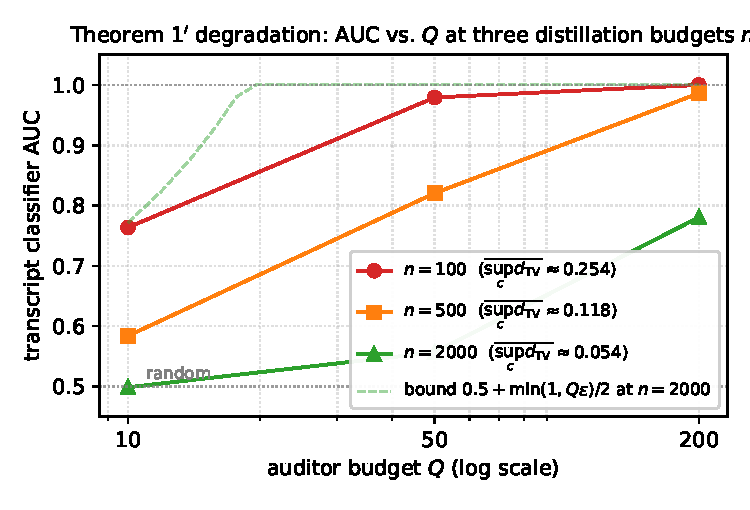
\includegraphics[width=0.78\linewidth]{toy-validation/auc-vs-Q.pdf}
\caption{Transcript-classifier AUC versus auditor budget $Q$ at three
distillation budgets $n$. Higher $n$ shrinks the per-context $\sup_c \dtv$ and
flattens the AUC curve: at $n = 2000$ ($\sup_c \dtv \approx 0.05$), $Q = 10$
yields random AUC; at $n = 100$ ($\sup_c \dtv \approx 0.26$), $Q = 200$ already
saturates. The dashed reference is the bound $0.5 + \min(1, Q\varepsilon)/2$
from Theorem~\ref{thm:approx} evaluated at $\varepsilon = \overline{\sup_c \dtv}$
for $n=2000$.}
\label{fig:auc-curve}
\end{figure}

\begin{table}[h]
\centering\small
\begin{tabular}{rrrrrr}
\toprule
$n$ & $Q$ & $\sup_c \dtv$ & $\overline{\dtv}$ & $Q \cdot \sup \dtv$ & AUC \\
\midrule
100  & 10  & 0.268 & 0.214 & 2.68  & 0.764 \\
100  & 50  & 0.239 & 0.207 & 11.95 & 0.979 \\
100  & 200 & 0.256 & 0.212 & 51.17 & 1.000 \\
\midrule
500  & 10  & 0.112 & 0.094 & 1.12  & 0.584 \\
500  & 50  & 0.119 & 0.094 & 5.95  & 0.821 \\
500  & 200 & 0.123 & 0.098 & 24.65 & 0.986 \\
\midrule
2000 & 10  & 0.060 & 0.049 & 0.60  & 0.499 \\
2000 & 50  & 0.051 & 0.045 & 2.53  & 0.557 \\
2000 & 200 & 0.052 & 0.044 & 10.46 & 0.781 \\
\bottomrule
\end{tabular}
\caption{Toy validation. $n$ samples per context distill the joint kernel; $Q$ is
the auditor budget; $\sup_c \dtv$ is the worst-case per-context TV between $K_G$
and $\hat K_G$; AUC is the held-out classifier AUC. Source data:
\texttt{paper/toy-validation/results.json}.}
\label{tab:toy-results}
\end{table}

\begin{enumerate}
  \item \emph{Distillation works}: increasing $n$ shrinks $\sup_c \dtv$ from
    $\approx 0.27$ at $n = 100$ to $\approx 0.05$ at $n = 2000$, consistent
    with the $O(m^2 \varepsilon^{-2} \log(|\C| m / \delta))$ rate of
    \Cref{prop:finite-alphabet}.
  \item \emph{The $Q\varepsilon$ shape is observable}: at fixed $n = 2000$,
    AUC moves from $0.499$ (random) at $Q = 10$ to $0.781$ at $Q = 200$,
    paralleling the bound's monotone-in-$Q$ growth.
  \item \emph{$Q\varepsilon \gg 1$ saturates}: at $n = 100$, $Q = 200$,
    $Q \cdot \sup \dtv \approx 51 \gg 1$, and the classifier achieves
    $\mathrm{AUC} = 1.000$. The $\min(1, Q\varepsilon)$ clipping in
    \Cref{thm:approx} is the relevant regime; classifier-class confounding
    cannot rescue indistinguishability once $Q\varepsilon$ is large.
\end{enumerate}

\paragraph{Caveats.}
Classifier AUC is a lower bound on TV-distinguishability subject to model-class
expressivity; an AUC near $0.5$ does not certify $\dtv \approx 0$ in general,
which is precisely why we report $\sup_c \dtv$ alongside AUC. The experiment
does not say anything about real LLM agents: $\C$ is finite, $\YR$ is finite,
the kernel is hand-built, and the auditor is non-adaptive. The intended message
is that \Cref{thm:transcript-indist}'s construction is tractable and that
\Cref{thm:approx}'s degradation shape matches a controlled simulation; all
inferential force comes from the theorem, not the experiment.

\end{document}
